\documentclass[11pt,letterpaper,notitlepage]{report}
\usepackage[latin1]{inputenc}
\usepackage{amsmath}
\usepackage{amsfonts}
\usepackage{amssymb}
\usepackage{fancyhdr}
\newcommand{\field}[1]{\mathbb{#1}}
\renewcommand{\labelenumi}{\alph{enumi})}
\usepackage{tikz}
\usepackage{fancybox}
\title{Minesweeper Solver Analysis}
\author{Brian Stack, bis12@case.edu}
\date{\today}
\usepackage[small,bf]{caption}
\usepackage{subfigure}
\usepackage{wrapfig}
\usepackage{fullpage}
\usepackage{tikz}
\usepackage{tikz-qtree}



\begin{document}
\maketitle
\section*{Analysis of Game}
\begin{enumerate}
\item 
\begin{align*}
C = \{ (V_1, V_2) &= V_1 + V_2 = 1,\\
       (V_3, V_4) &= V_3 + V_4 = 1,\\
       (V_1, V_2, V_3, V_4, V_5) &= V_1 + V_2 + V_3 + V_4 + V_5 = 2\}
\end{align*}
\item ~\\
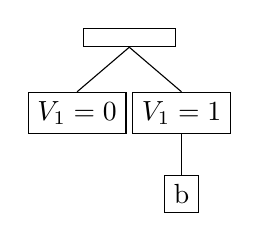
\begin{tikzpicture}
\tikzstyle{every node}=[rectangle,draw]
\Tree [.~~~~~~~~~ [.{$V_1 = 0$}  ] [.{$V_1 = 1$} b ] ]
\end{tikzpicture}
\end{enumerate}
\section*{Observations on Solutions}
\begin{enumerate}
\setcounter{enumi}{2}
\item ababab
\end{enumerate}
\end{document}





